% ****** Start of file apssamp.tex ******
%
%   This file is part of the APS files in the REVTeX 4.1 distribution.
%   Version 4.1r of REVTeX, August 2010
%
%   Copyright (c) 2009, 2010 The American Physical Society.
%
%   See the REVTeX 4 README file for restrictions and more information.
%
% TeX'ing this file requires that you have AMS-LaTeX 2.0 installed
% as well as the rest of the prerequisites for REVTeX 4.1
%
% See the REVTeX 4 README file
% It also requires running BibTeX. The commands are as follows:
%
%  1)  latex apssamp.tex
%  2)  bibtex apssamp
%  3)  latex apssamp.tex
%  4)  latex apssamp.tex
%
\documentclass[%
 reprint,
%superscriptaddress,
%groupedaddress,
%unsortedaddress,
%runinaddress,
%frontmatterverbose,
%preprint,
%showpacs,preprintnumbers,
%nofootinbib,
%nobibnotes,
%bibnotes,
 amsmath,amssymb,
 aps,
%pra,
%prb,
%rmp,
%prstab,
%prstper,
%floatfix,
]{revtex4-1}

\usepackage[utf8]{inputenc}
\usepackage[norsk]{babel}
\usepackage{graphicx}% Include figure files
\usepackage{dcolumn}% Align table columns on decimal point
\usepackage{bm}% bold math
\usepackage[mathlines]{lineno}% Enable numbering of text and display math
%\linenumbers\relax % Commence numbering lines

\usepackage[usenames,dvipsnames,svgnames,table]{xcolor}
\usepackage[colorlinks]{hyperref}
\usepackage{relsize}
\usepackage{amsmath,graphicx,varioref,verbatim,amsfonts,geometry}
\newcommand*\diff{\mathop{}\!\mathrm{d}}
\newcommand*\Diff[1]{\mathop{}\!\mathrm{d^#1}}
\usepackage{ulem}
\usepackage{amssymb}
\usepackage{soul}
\usepackage{dsfont}
\usepackage{commath}
\usepackage{wrapfig}
\usepackage[free-standing-units=true]{siunitx}
\DeclareSIUnit\year{yr}
\usepackage{gensymb}
\newcommand{\ROM}[1]{%
  \textup{\uppercase\expandafter{\romannumeral#1}}%
}
\usepackage{physics}
\usepackage{caption}
\usepackage{bm}

%\usepackage[showframe,%Uncomment any one of the following lines to test
%%scale=0.7, marginratio={1:1, 2:3}, ignoreall,% default settings
%%text={7in,10in},centering,
%%margin=1.5in,
%%total={6.5in,8.75in}, top=1.2in, left=0.9in, includefoot,
%%height=10in,a5paper,hmargin={3cm,0.8in},
%]{geometry}

\begin{document}

%\preprint{APS/123-QED}

\title{Strøm og Spenning}

\author{\textsc{Haugerud, Ivar Svalheim}}
\affiliation{%
 University of Oslo\\
}%

\date{\today}

\begin{abstract}
We need to test if our system behaves as it should based on the equations we have in the theory section, which is derived in the appendix. To start with this we visualized the particles in the compartment. Since the visualizing demands more computer power than our computers can handle here at the university of Soby, we had to limit ourselves to only $100$ particles. We saw that the particles behaved as they should, and did bounce on the walls when they were meant to, and it looked like their kinetic energy was conserved.
\end{abstract}

\pacs{Valid PACS appear here}% PACS, the Physics and Astronomy
                             % Classification Scheme.
%\keywords{Suggested keywords}%Use showkeys class option if keyword
                              %display desired
\maketitle

%\tableofcontents

\section{\label{teori}Teori}
Vi jobber med elektriske kretser hvor vi bruker Ohm's lov \cite{skaar} for å regne på kretsene våre
\begin{equation}
  V = IR \label{ohm},
\end{equation}
hvor $V$ er spenningsfallet over en komponent, $I$ er strømmen som gjør gjennom komponenten, og $R$ er resistansen til komponenten. Dette gir oss forholdet mellom motstand, strøm og spenningsfall, som er nødvendig for en hver krets. Denne formelen kommer vi til å bruke mye gjennom forsøket siden vi kan finne resistansen ved å måle spenningsfallet over en komponent når vi vet hva strømmen er. Dette blir spesielt nyttig hvis resistansen til en komponent er avhengig av temperaturen i rommet. \\
I kretsene våre kommer vi til å bruke kondensatorer. Kondensatorer kan lagre elektriske ladninger med netto ladning $Q$, dette generer et spenningsforskjell mellom kondensatorplatene $V$. Disse to egenskapene til kondensatoren gir oss kapasitansen til kondensatoren som er gitt av
\begin{equation}
  C = \frac{Q}{V},
\end{equation}
hvor $C$ er kapsitansen. Kapasitansen er bare avhengig av materialet og de geometriske strørrelsene til kondensatorplatene \cite{skaar}. Kapasitansen sier oss hvor mye ladning kondensatoren klarer å oppbevare før den blir \textit{full}. Hvis man kobbler inn en resistanse i kretsen også, slik at man får en RC-krets, vil man ha lagd et lavpassfilter. Grunnen til dette er at forflyttingen av ladninger i kretsen tar tid, og gjør at, hvis man har en vekselstrøm (AC) vil spenningen over kondensatoren være en funksjon av tid, og med for stor frekvens på strømmen vil ikke strømmen i kretsen ha tid til å fylle opp kondensatoren med ladninger før strømmen endres igjen. Og derfor vil man ha en høy frekvens som går inn i kondensatoren, men en lav frekvens som går ut av kondensatoren. Forholdet mellom spenningen inn $V_i$ og spenningen ut $V_u$ kan vises at \cite{oppgave} er
\begin{equation}
  \abs{\frac{V_u}{V_i}} = \frac{1}{\sqrt{1+\left(\frac{\omega}{\omega_0}\right)^2}}
\end{equation}som, ved å ta logarytmen på begge sider, kan skrives om til
\begin{equation}
  \log\abs{\frac{V_u}{V_i}} = -\frac{1}{2}\log\left\{1+\left(\frac{\omega}{\omega_0}\right)^2 \right\}
\end{equation}
Her har spenningen inn en frekvens $\omega$ og $\omega = 1/RC$, som er den karakteristiske frekvens til kretsen. For lave frekvenser ser vi at $\log\abs{V_u/V_i}\approx 0$. For høye frekvenser ser vi at $\log\abs{V_u/V_i}\approx -\log(\omega) + log(\omega_0)$, som, hvis plottet med logaritmiske akser, er en rett linje med konstantledd $\log(\omega_0)$ og stigningstall $-1$, der $x$-aksen er $\omega$ og $y$-aksen er $\abs{V_u/V_i}$. Dette betyr at den relative amplituden faller en faktor $10$ for hver faktor $10$ vi øker frekvensen. Dette gjør at de høye frekvensene vil falle bort, som gjøre kretsen til et lavpassfilter.

\section{\label{metode1}Metode}
Vi ønsket å finne ut hvordan det å måle motstand, strøm eller spenning påvirker kretsen som måleapparatet er med i. For å gjøre dette brukte vi to multimetere Fluke $75$ (F$75$) som er et håndholdt multimeter, og Fluke $45$ (F$45$), som er et stasjonert multimeter. Vi lot multimeterene måle på hverandre i en ekstremt simpel krets der måleapparatene er de eneste komponentene i kretsen, dette er vist i figur \vref{fig1}. Dette gjorde vi for alle kombinasjonene av resistans, strøm og spenning i kretsen, og varierte sensitiviteten og samplings-frekvensen (slow (S), medium (M) og fast (F)) til måleapparatene. \\
\begin{figure}[h!]
    \centering
    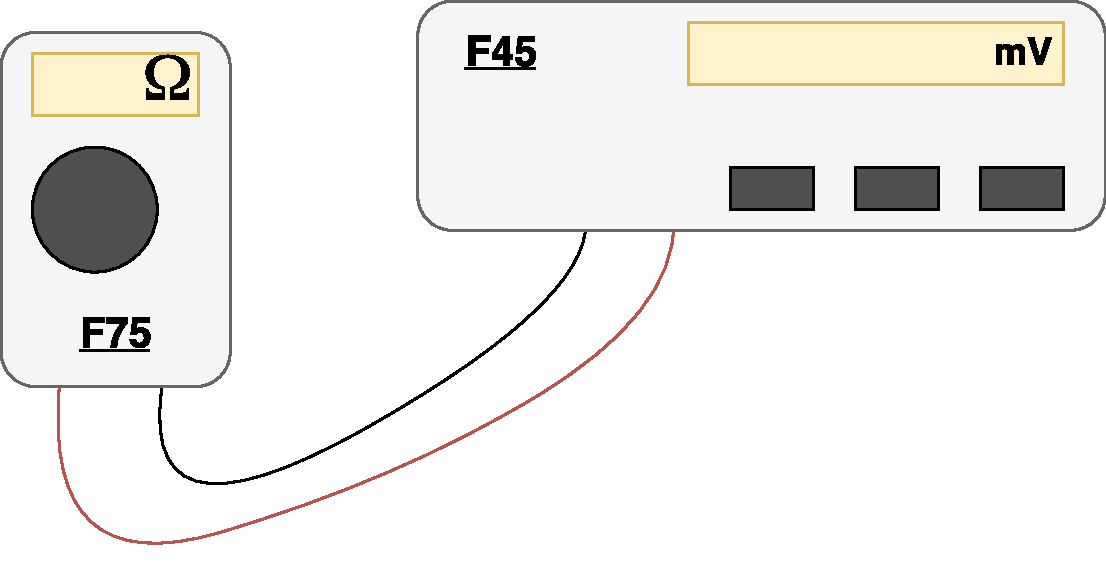
\includegraphics[scale=0.35]{fig_1.pdf}
    \caption{Figur som viser F$45$ og F$75$ som måler på hverandre i en veldig simpel krets. I dette eksempelet måler F$75$ resistansen gjennom kretsen, mens F$45$ måler spenningen.}
    \label{fig1}
\end{figure}
Nå som vi viste hvordan måleapparatene påvirket krets de selv er med i brukte vi dem til å måle resistansen til to motstander hvor vi vist den eksakte verdien av resitansen. Dette gjorde vi ved å sette opp en enkel krets vist i figur \vref{fig2} ved hjelp av et breadbord.
\begin{figure}[h!]
    \centering
    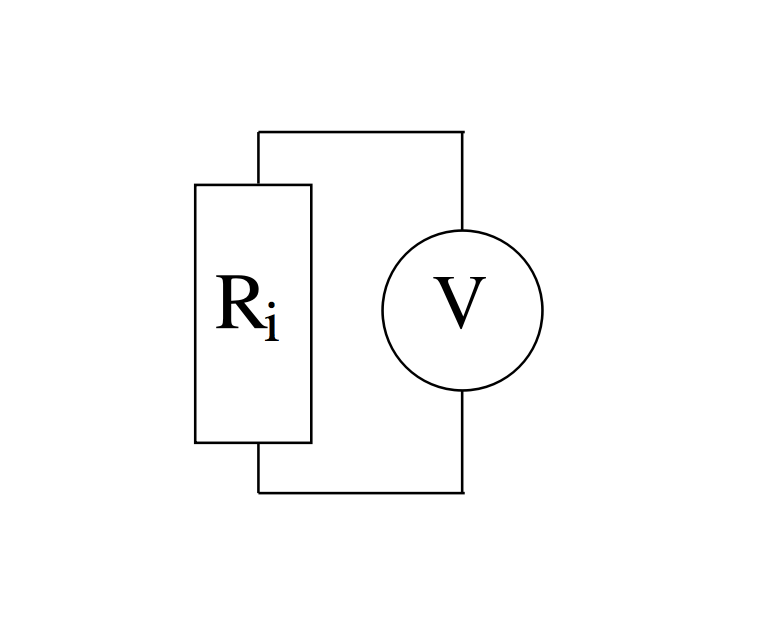
\includegraphics[scale=0.15]{fig_2.png}
    \caption{Krets brukt for å måle resistansen til motstander der vi kunne variere $R_i$.}
    \label{fig2}
\end{figure}
Vi valgte denne kretsen siden dette var den letteste mulige kretsen for hensikten vår. Vi brukte to forskjellige resistanser i kretsen, først $R_1 \sim 10 \Omega$ og så $R_2 \sim 1 M\Omega$. Vi gjorde først målingene med F$75$ og så med F$45$. Hvor begge appartene brukt ohm-funksjonen, slik at de genererte strømmen i kretsen selv.\\
Vi ønsket så å utvide kretsen og gjøre den litt mer komplisert. Kretsen vi lagde er vist i figur \vref{fig_3}.
\begin{figure}[h!]
    \centering
    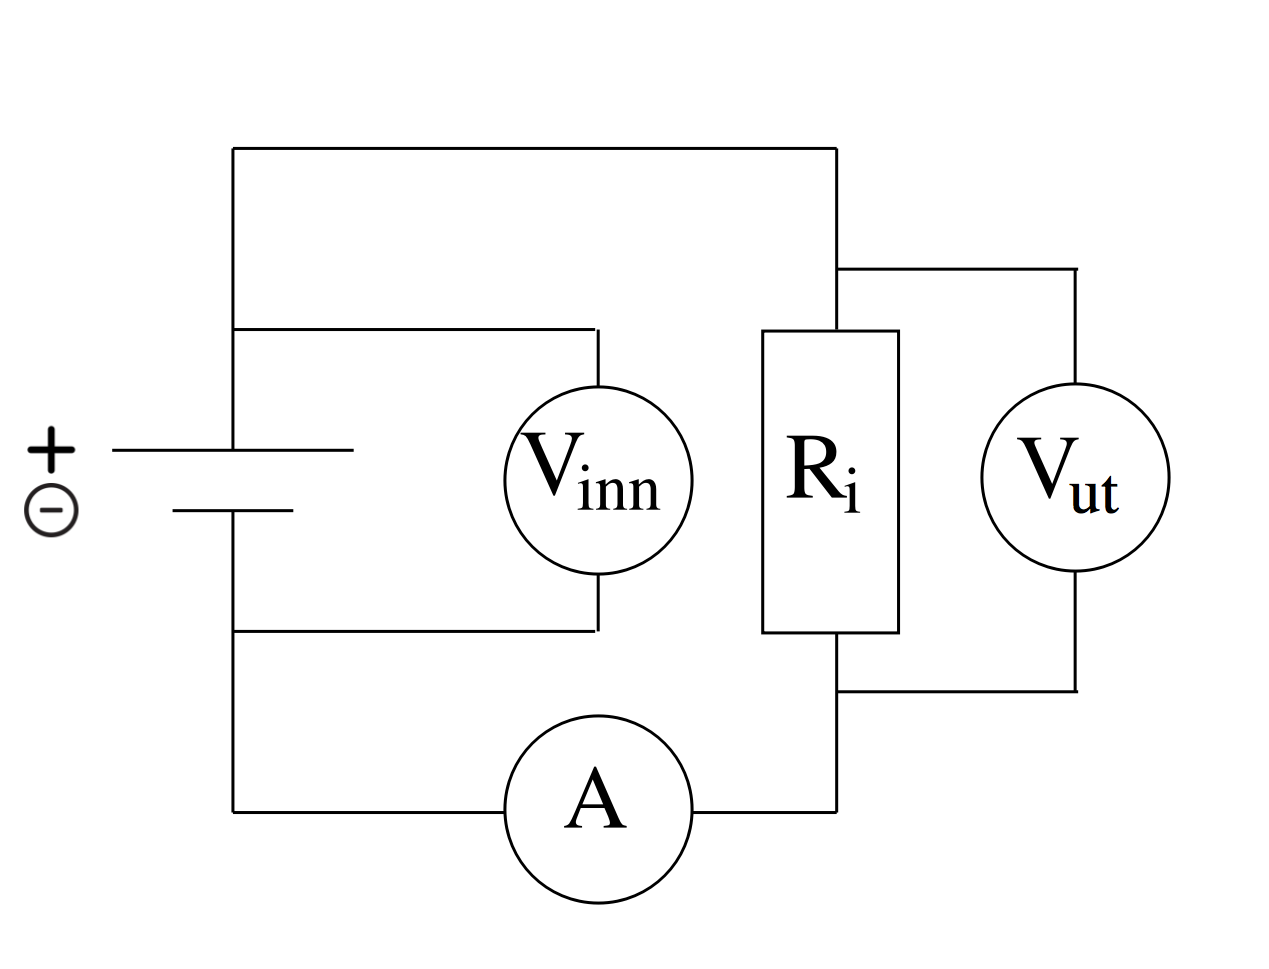
\includegraphics[scale=0.15]{fig_3.png}
    \caption{Krets brukt for å måle resistansen til motstander der vi kunne variere $R_i$.}
    \label{fig2}
\end{figure}
I denne kretsen måler vi spenningsfallet over hele kretsen ved $V_{in}$, spenningsfallet over resistansen ved $V_{ut}$, og strømmen som går gjennom kretsen ved amperemeteret. Med disse målingene kan vi regne ut resistansen til motstandene. Siden vi hadde to mutlimetere, og tre verdier vi ønsket å måle i kretsen måtte vi koble om kretsen under forsøket for å gjøre de forskjellige målingene. Når alt var riktig koblet opp varierte vi strømmen i kretsen, og gjorde målinger for begge resistanser for hver frekvens. I kretsen vår brukte vi F$45$ som $V_{inn}$ og $V_{ut}$, mens vi brukte F$75$ som ampere meter, grunnen til dette var at det ga oss minst omkoblinger underveis.

\begin{thebibliography}{9}
\bibitem{squires}
Squires, G.L. \emph{Practical Physics}, Cambridge University Press, 2001.
\bibitem{skaar}
Skaar, J. \emph{Elektromagnetisme}, 2017
\bibitem{oppgave}
Dysthe, D.K\,\, Røyne, A.\,\, Ulven, O.I \emph{Strøm og spenning}, 2018
 \end{thebibliography}

\end{document}
%
% ****** End of file apssamp.tex ******
